 \section{Introduci\'on}
	\subsection{Objetivo}
		\setlength{\parindent}{1em}
		\setlength{\parskip}{10pt}
			El alumno realizar\'a una ALU,la que incluir\'a registros de corrimientos, l\'ogicos y aritm\'eticos la cual podr\'a realizar las operaciones con datos de 'n' bits especificados, tendr\'a una terminal que sirva para el control de carga.
	\subsection{Introducci\'on te\'orica}
		\subsubsection{Unidad Aritmetica L\'ogica (ALU)}
			La ALU es la parte de la computadora que realiza las operaciones l\'ogicas y aritmeticas de los datos. Todos los dem\'as elementos de los sistemas de computadoras (Control Unit, Registros, memoria, entrada/salida) son algunos de los datos que se le entregan a la ALU para que los procese y despu\'es los devuelva. Entonces, en un sentido, hemos alcanzado la esencia de una computadora cuando consideramos una ALU.
\vskip 1pt
	Una ALU y, en realidad todos los componentes electronicos en una computadora estan basados en el uso de simples dispositivos l\'ogicos digitales simples que pueden guardar digitos binarios y realizar simples operaciones l\'ogicas boleanas.
\vskip 1pt
	En la siguiente figura se muestra en t\'erminos generales, como esta interconectada la ALU con el resto del procesador. Los datos son presentados en los registros de la ALU, y los resultados de la operaci\'on se guarda en los registros. Estos registros son almacenados temporalmente mientras el procesador este conectado por rutas de se\~nal al ALU. Al ALU tambi\'en se le pueden configurar banderas como el resultado de una operaci\'on. Por ejemplo, la bandera de overflow se configura en 1 si el resultado excede el tama\~no del registro en donde va a ser almacenado. Los valores de estas banderas tambi\'en son almacenadas en los registros dentro del procesador. La unidad de control nos provee se\~nalesque controlan la operaci\'on del ALU y el movimiento de datos de entrada y salida del ALU.
	\begin{figure}[h]
			\centering		
			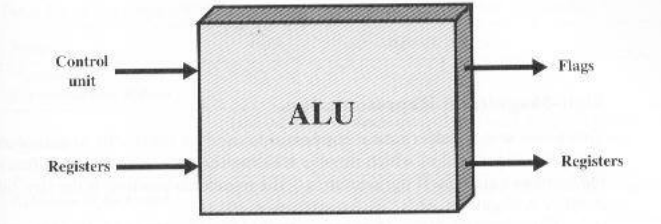
\includegraphics[width=\textwidth]{IOALU}
			\caption{Entradas y Salidas del ALU}
	\end{figure}
	\subsubsection{?`Qu\'e es VHDL?}
		VHDL es un lenguaje de dise\~no de software destinado a usarse en todas las fases del dise\~no de sistemas digitales. VHDL viene de VHSIC (Very High Speed Integrated Circuits) lenguaje descriptor de hardware. Su desarrollo empez\'o en 1983 con un contrato por parte del departamento de defenza de los Estados Unidos de \'America, y se volvi\'o un est\'andar de la IEEE en 1987.
	\subsubsection{?`Qu\'e es una FPGA?}
Una FPGA (Field Programmable Gate Array) es un complejo circuito integrado digital programable compuesto por bloques l\'ogicos configurables (CLB) y puertos de entrada/salida (IOB), cuya interconexi\'on y funcionalidad puede ser programada mediante un lenguaje de descripci\'on especializado.
\vskip 1pt
Su principal caracter\'istica y ventaja es que pueden reprogramarse para un trabajo espec\'ifico o cambiar sus requisitos despu\'es de haberse fabricado. Esto tambi\'en implica que en muchos casos se pueden hacer cambios f\'isicos sin hacer modificaciones costosas en la placa que lo soporta.
\vskip 1pt
B\'asicamente, una FPGA es un conjunto de m\'ultiples circuitos (l\'ogicos y de otros tipos) dispuestos matricialmente, cuyas interconexiones son programables por el usuario para la aplicaci\'on requerida. En una FPGA se programa su hardware, a diferencia de los microcontroladores / microprocesadores, en los que solo existe un hardware fijo y se programa su software (firmware).
\vskip 1pt
Hist\'oricamente, las FPGA fueron inventadas en el a\~no 1984 por Ross Freeman y Bernard Von Der Schmitt, cofundadores de la empresa Xilinx, fabricante de las mismas. Como resultado de numerosas evoluciones, la compa\~n\'ia produjo la primera familia de dispositivos l\'ogicos programables por el usuario, de prop\'osito general.
\vskip 1pt
Las FPGA, adem\'as de contener puertas l\'ogicas AND y OR, tienen memoria RAM, controladores de reloj, etc., por lo que son muy apropiadas para el dise\~no de sistemas embebidos con microprocesador. La compa\~n\'ia Xilinx ha evolucionado dicha tecnolog\'ia hasta convertirla en un nuevo concepto a tener en cuenta en ciertos entornos de trabajo.
	\subsection{Material y Equipo Empleado}
		\begin{itemize}
			\item 1 FPGA
			\item 1 Tarjeta de evaluaci\'on de pruebas \'o Protoboard microswitches con resistencias 10 KoHms, 20 leds con resistencias 330 oHms, 1 display de 4 digitos multiplexado de \'anodo com\'un.
			\item 1 eliminador de celular de 5v con cable mini usb.
			\item Quartus Prime Lite
		\end{itemize}
	